% Options for packages loaded elsewhere
\PassOptionsToPackage{unicode}{hyperref}
\PassOptionsToPackage{hyphens}{url}
%
\documentclass[
]{article}
\usepackage{amsmath,amssymb}
\usepackage{lmodern}
\usepackage{listings}
\usepackage{graphicx}
\usepackage{iftex}
\ifPDFTeX
  \usepackage[T1]{fontenc}
  \usepackage[utf8]{inputenc}
  \usepackage{textcomp} % provide euro and other symbols
\else % if luatex or xetex
  \usepackage{unicode-math}
  \defaultfontfeatures{Scale=MatchLowercase}
  \defaultfontfeatures[\rmfamily]{Ligatures=TeX,Scale=1}
\fi
% Use upquote if available, for straight quotes in verbatim environments
\IfFileExists{upquote.sty}{\usepackage{upquote}}{}
\IfFileExists{microtype.sty}{% use microtype if available
  \usepackage[]{microtype}
  \UseMicrotypeSet[protrusion]{basicmath} % disable protrusion for tt fonts
}{}
\makeatletter
\@ifundefined{KOMAClassName}{% if non-KOMA class
  \IfFileExists{parskip.sty}{%
    \usepackage{parskip}
  }{% else
    \setlength{\parindent}{0pt}
    \setlength{\parskip}{6pt plus 2pt minus 1pt}}
}{% if KOMA class
  \KOMAoptions{parskip=half}}
\makeatother
\usepackage{xcolor}

\setlength{\emergencystretch}{3em} % prevent overfull lines
\providecommand{\tightlist}{%
  \setlength{\itemsep}{0pt}\setlength{\parskip}{0pt}}
\setcounter{secnumdepth}{-\maxdimen} % remove section numbering
\ifLuaTeX
  \usepackage{selnolig}  % disable illegal ligatures
\fi
\IfFileExists{bookmark.sty}{\usepackage{bookmark}}{\usepackage{hyperref}}
\IfFileExists{xurl.sty}{\usepackage{xurl}}{} % add URL line breaks if available
\urlstyle{same} % disable monospaced font for URLs
\hypersetup{
  hidelinks,
  pdfcreator={LaTeX via pandoc}}

  
  \definecolor{codegreen}{rgb}{0,0.6,0}
  \definecolor{codegray}{rgb}{0.5,0.5,0.5}
  \definecolor{codepurple}{rgb}{0.58,0,0.82}
  \definecolor{backcolour}{rgb}{0.95,0.95,0.92}
  
  \lstdefinestyle{mystyle}{
      backgroundcolor=\color{backcolour},   
      commentstyle=\color{codegreen},
      keywordstyle=\color{magenta},
      numberstyle=\tiny\color{codegray},
      stringstyle=\color{codepurple},
      basicstyle=\ttfamily\footnotesize,
      breakatwhitespace=false,         
      breaklines=true,                 
      captionpos=b,                    
      keepspaces=true,                 
      numbers=left,                    
      numbersep=5pt,                  
      showspaces=false,                
      showstringspaces=false,
      showtabs=false,                  
      tabsize=2
  }
  
  \lstset{style=mystyle}

  \graphicspath{ {./ } }


\title {Maze Master \\[1ex] \large Dokumentacja implementacyjna \\[1ex] https://github.com/JGolaszewski/MazeMaster}
\date{\today}
\author{Jędrzej Gołaszewski i Szymon Stasiak}


\begin{document}
\pagenumbering{gobble}  
\maketitle
\newpage
\pagenumbering{arabic}

\hypertarget{funkcjonalnoux15bux107-programu}{%
\section{\texorpdfstring{Funkcjonalność programu
}{Funkcjonalność programu }}\label{funkcjonalnoux15bux107-programu}}

Celem tego programu jest umożliwienie użytkownikowi znalezienia
najkrótszej ścieżki przez labirynt, który został stworzony na podstawie
pliku wygenerowanego na stronie http://tob.iem.pw.edu.pl/maze/. Program
wygeneruje precyzyjny ciąg instrukcji, który prowadzi od punktu
początkowego do punktu wyjściowego. Dzięki niemu użytkownik może
sprawnie i efektywnie odnaleźć właściwą drogę.

\hypertarget{uux17cytkowanie}{%
\section{Użytkowanie}\label{uux17cytkowanie}}

Ten program służy do rozwiązywania labiryntów zapisanych w plikach
tekstowych. Rozwiązanie jest zapisywane do innego pliku tekstowego lub
wyświetlane w konsoli, jeśli nie zostanie podany plik wyjściowy.

./bin -i \textless plik\_wejściowy\textgreater{} {[}-o
\textless plik\_wyjściowy\textgreater{]} {[}opcje{]}

\hypertarget{argumenty-programu}{%
\subsubsection{Argumenty programu}\label{argumenty-programu}}

-i \textless plik\_wejściowy\textgreater{} lub -in
\textless plik\_wejściowy\textgreater: Określa nazwę pliku tekstowego
zawierającego labirynt do rozwiązania.

-o \textless plik\_wyjściowy\textgreater{} lub -out
\textless plik\_wyjściowy\textgreater: Określa nazwę pliku tekstowego,
do którego program zapisze rozwiązanie labiryntu. Jeśli ta opcja nie
zostanie podana, rozwiązanie zostanie wyświetlone w konsoli.

-v lub -verbose: Włącza wyświetlanie dodatkowych informacji podczas
działania programu.

-d lub -debug: Włącza tryb debugowania, umożliwiając analizę
szczegółowych informacji na temat działania programu.

-h lub -help: Wyświetla pomoc dotyczącą sposobu użycia programu.

-q lub -quit: Natychmiastowe wyjście z programu.

\hypertarget{architektura-systemu}{%
\section{Architektura Systemu}\label{architektura-systemu}}

System na jakim działa, systemowe funkcje jakies ewentualnie podzial na
pliki programu, jezyk w jakim jest napisany wersja jezyka (c2x), foldery
wejście wyjście bin itp

\hypertarget{ux15brodowisko-uruchomieniowe}{%
\subsubsection{Środowisko
uruchomieniowe}\label{ux15brodowisko-uruchomieniowe}}

Program jest przystosowany do działania w środowisku Unixowym

Testy programu były prowadzone w:

Subsystem Kali Linux for Windows 11

Linux Ubuntu

\hypertarget{wersja-c}{%
\subsubsection{\texorpdfstring{Wersja C }{Wersja C }}\label{wersja-c}}

Program jest napisany w języku programowania C w standardzie C23 (C2X);

\hypertarget{makefile}{%
\subsubsection{Makefile}\label{makefile}}

Ten Makefile jest narzędziem do automatyzacji procesu kompilacji
programu napisanego w języku C. Składa się z trzech głównych celów:
"build", "clean" i "test". Cel "build" kompiluje pliki źródłowe do pliku
wykonywalnego, przy użyciu zdefiniowanych flag kompilacji. "Clean" usuwa
plik wykonywalny, a "test" uruchamia program z określonymi argumentami w
celu przetestowania go. Zmienne definiują nazwę pliku wykonywalnego,
katalog wyjściowy i parametry kompilacji. Makefile ten zapewnia prosty i
elastyczny sposób zarządzania procesem kompilacji i testowania programu
w języku C.

\hypertarget{opis-plikuxf3w}{%
\subsubsection{Opis plików}\label{opis-plikuxf3w}}

\hypertarget{pliki-wejux15bciowe}{%
\paragraph{Pliki Wejściowe:}\label{pliki-wejux15bciowe}}

\begin{itemize}
\item
  Plik binarny
\end{itemize}

Plik binarny zawiera nagłówek pliku, sekcje kodującą, nagłówek sekcji
kodowania oraz sekcja wyniku.

Nagłówek pliku składa się z :

\begin{itemize}
\item
  32 bitów id pliku(0x52524243)
\item
  8 bitów znak ESC
\item
  Liczba kolumn 16 bitów
\item
  Liczba linii 16 bitów
\item
  Pozycja x wejścia 16 bitów
\item
  Pozycja y wejścia 16 bitów
\item
  Pozycja x wyjścia 16 bitów
\item
  Pozycja y wyjścia 16 bitów
\item
  Pamięć zarezerwowaną 96 bitów
\item
  Licznik słów kodowych 32 bitów
\item
  Wskaźnik na rozwiązanie 32 bitów
\item
  Początek słowa kodowego (Separator) 8 bitów
\item
  Definicja ściany labiryntu 8 bitów
\item
  Definicja ścieżki labiryntu 8bitów
\end{itemize}

\begin{quote}
W sumie: 420 bitów

Slowa kodowe:
\end{quote}

\begin{itemize}
\item
  Separator 8 bitów
\item
  Wartość 8 bitów (Ściana / Ścieżka)
\item
  Liczba wystąpień 8 bitó (0 -- to jedno wystąpienie)
\end{itemize}

Nagłówek rozwiązania:

\begin{itemize}
\item
  Id sekcji rozwiązania 32 bitów (0x52524243)
\item
  Liczba kroków do przejścia 8 bitów (0 -- to jeden krok)
\end{itemize}

W sumie 40 bitów

Krok rozwiązania:

\begin{itemize}
\item
  Kierunek 8 bitów (N, E, S, W)
\item
  Licznik pól do przejścia (0 -- to jedne pole)
\end{itemize}

\begin{itemize}
\item
  Plik tekstowy
\end{itemize}

Plik tekstowy zawiera labirynt zapisany tekstowo gdzie jeden znak
odpowiada jednemu polu na siatce labiryntu. Znak `\#' - odpowiada
ścianie labiryntu a ` ' - odpowiada ścieżce labiryntu, `K' - odpowiada
końcu a `P' - odpowiada początkowi.

Przykładowy plik labiryntu:

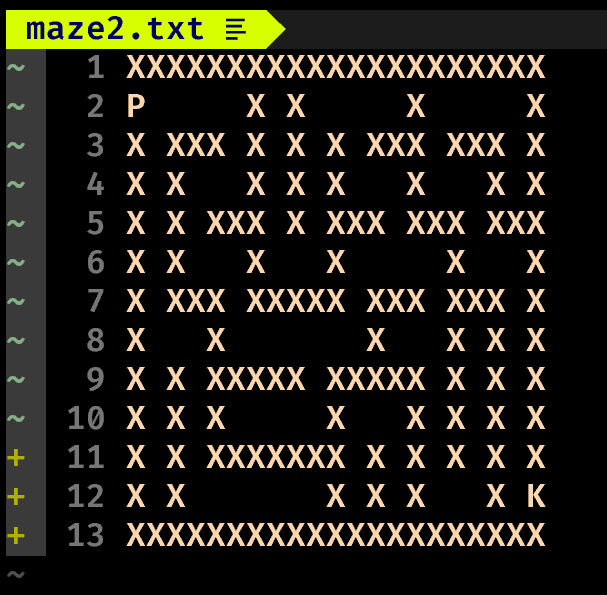
\includegraphics[width=5cm, height=5cm]{plik.png}


\hypertarget{pliki-programu}{%
\paragraph{Pliki programu:}\label{pliki-programu}}

\begin{itemize}
\item
  main.c
\end{itemize}

Main łączy moduły programu w spójną całość.

\begin{itemize}
\item
  graph.c oraz graph.h
\end{itemize}

Zawiera implementację struktury wierzchołków oraz funkcje służące do
odczytu ich z \hyperref[pliki-tymczasowe] {tymczasowego node\_temp}

\begin{itemize}
\item
  BFS.c, BFS.h, readPath.c oraz readPath.h
\end{itemize}

Zawiera implementację  \hyperref[bfs]{modułu BFS} wraz z
odczytywaniem rozwiązania.

\begin{itemize}
\item
  interface.c, interface.h oraz reports.h
\end{itemize}

Zawiera implementację modułu komunikacji z użytkownikiem 
oraz \hyperref[moux17cliwe-bux142ux119dy]{makra do zgłaszania błędów}.

\begin{itemize}
\item
  parser.c oraz parser.h
\end{itemize}

Zawiera implementację \hyperref[parser]{modułu parsera}który
zamienia plik labiryntu na grafowy jego odpowiednik.

\begin{itemize}
\item
  Macros.h
\end{itemize}
\hyperref[staux142e-programu-i-funkcje-pomocnicze]{Zawiera makra stałych w programie i funkcje pomocnicze.} 

\hypertarget{struktury-programu}{%
\subsubsection{Struktury programu}\label{struktury-programu}}

W programie wykorzystywane są dwie struktury własne

\begin{itemize}
\item
  Node (node\_t)
\end{itemize}

Struktura node opisuje wierzchołek grafu (kafelek ścieżki w labiryncie).

W jej skład wchodzą zmienne: x (położenie x), y (położenie y),
adj(zmienna trzymająca połączenia z kolejnymi wierzchołkami w sposób
bitowy tzn.: od lewej 1 bit przejście w lewo, 2 bit przejście w prawo, 3
bit przejście w górę, 4 bit przejście w dół).

Implementacja struktury wygląda następująco:

\begin{lstlisting}[language=C, caption=Struktura Node]
  enum Direction {
    LEFT = 0b00,
    RIGHT = 0b01,
    TOP = 0b10,
    BOTTOM = 0b11
};

typedef struct Node {
    USHORT x : 12;
    USHORT y : 12;
    //ADJ - adjacency of node BITS: (LEFT)(RIGHT)(TOP)(BOTTOM)
    UCHAR adj : 4;
    // 00 - LEFT   01 RIGHT  10 - TOP  11 - BOTTOM
    UCHAR parent : 2;
    UCHAR flag : 1;
} node_t;
\end{lstlisting}

\begin{itemize}
\item
  Queue (queue\_t)
\end{itemize}

Struktura queue jest wrapperem na wskaźnik na plik(jest to plik
tymczasowy w którym są przetrzymywane dane kolejki) poszerzona o 1 bit
utrzymujący informację o tym czy kolejka jest aktualnie pusta.

Implementacja struktury wygląda następująco:

\begin{lstlisting}[language=C, caption=Struktura Queue]
  typedef struct Queue {
    FILE* queueData;
    UCHAR isEmpty : 1;
} queue_t;
\end{lstlisting}

\hypertarget{zaux142oux17cenia-i-rozwiux105zania-systemu}{%
\section{Założenia i rozwiązania
systemu}\label{zaux142oux17cenia-i-rozwiux105zania-systemu}}

\hypertarget{przygotowanie-danych-do-algorytmu}{%
\subsubsection{\texorpdfstring{Przygotowanie danych do algorytmu
}{Przygotowanie danych do algorytmu }}\label{przygotowanie-danych-do-algorytmu}}

Dane z \hyperref[pliki-wejux15bciowe]{pliku txt}  zawierające opis labiryntu są
przetwarzane na formę grafu. Każde pole jest przetwarzane na osobny
wierzchołek i przechowywane na siatce o rozmiarach x*y gdzie x to ilość
kolumn labiryntu a y ilość wierszy. Każdy element nawet pole ze ściana
ma swój wierzchołek jednak pola ściany są pojedynczymi wierzchołkami bez
żadnych krawędzi.\\
Pola puste labiryntu te po których możemy chodzić posiadają opis w
formie bitowej opisujących ich sąsiadów to znaczy możemy się z tego
dowiedzieć w którym kierunku możemy pójść dalej do góry do dołu w prawo
czy na lewo. Opis ten jest tworzony podczas \hyperref[parser]{parsowania}.

\hypertarget{uux17cyty-algorytm}{%
\subsubsection{Użyty algorytm}\label{uux17cyty-algorytm}}

BFS (Breadth-First Search) w rozwiązywaniu labiryntów

Algorytm rozwiązujący labirynt opiera się na BFS (Breadth-First Search),
ponieważ jest to efektywna metoda znajdowania najkrótszej ścieżki w
grafie nieskierowanym lub skierowanym, co jest istotne w przypadku
poszukiwania wyjścia z labiryntu.

Kroki algorytmu:

Inicjalizacja: Rozpoczynamy od wierzchołka, który jest znanym wyjściem z
labiryntu.

Przeszukiwanie: Wykonujemy algorytm BFS, sprawdzając kolejne wierzchołki
labiryntu.

Oznaczanie kierunku: Podczas sprawdzania kolejnych wierzchołków grafu,
oznaczamy kierunek, z którego przyszliśmy do danego wierzchołka. Dzięki
temu będziemy mieli informację o ścieżce prowadzącej do danego
wierzchołka.

Znalezienie wejścia: Kontynuujemy algorytm BFS aż do momentu znalezienia
wejścia do labiryntu. Gdy to nastąpi, mamy pełną informację o ścieżce
prowadzącej od wyjścia do wejścia.

Generowanie instrukcji: Znając ścieżkę od wyjścia do wejścia, możemy
generować instrukcje krok po kroku, które należy wykonać, aby przejść
przez labirynt.

\hypertarget{metoda-parsowania}{%
\subsubsection{Metoda parsowania}\label{metoda-parsowania}}

Metoda parsowania opiera się na zapisaniu wczytanych danych w sposób
binarny jako poszczególne kolejne trzy wiersze z pliku następnie
zidentyfikowanie połączeń pomiędzy pustymi polami i zapisanie ich
zgodnie z formatem pliku  \hyperref[pliki-tymczasowe] { temp\_nodes}.

Zamiana binarna odbywa się poprzez zamianę poszczególnych znaków w \hyperref[pliki-wejux15bciowe]{pliku
wejściowym} na ich bitowe reprezentacje (0
-- wolna przestrzeń, 1 - ściana). Po wczytaniu 3 pierwszych wierszy
program przystępuje do zamiany ich w bardziej czytelną formę krawędzi
grafu. Jeżeli znak jest 0 sprawdza on połączenia we wszystkie 4 kierunki
następnie zapisuje je do pliku tymczasowego \hyperref[pliki-tymczasowe] { temp\_nodes}
 wraz z przestrzenia na zapis flagi odwiedzenia
oraz kierunku rodzica. Następnie program zwalnia pamięć pierwszego
wiersza i wczytuje kolejny powtarzając proces aż do wyczerpania wierszy
w pliku.

\hypertarget{pliki-tymczasowe}{%
\subsubsection{Pliki tymczasowe}\label{pliki-tymczasowe}}

Program korzysta z 2 różnych plików tymczasowych aby ograniczyć zużycie
pamięci procesora do maksymalnie 512 kB.

\begin{itemize}
\item
  Plik ``temp\_nodes''
\end{itemize}

\begin{itemize}
\item
  Zastosowanie:
\end{itemize}

\begin{quote}
Przetrzymuje dane wierzchołka grafu ( adj -- 4 bity na możliwe kierunki
przejścia, flag -- 1 bit na flagę odwiedzenia, parent -- 2 bity na
kierunek w którym jest rodzic wierzchołka).
\end{quote}

\begin{itemize}
\item
  Struktura:
\end{itemize}

\begin{quote}
W pliku dane zapisywane są w sposób binarny po kolei od lewej do prawej,
z góry na dół. Każda ściana z pliku jest odzwierciedlona jako pusta
przestrzeń o rozmiarze wierzchołka a każda ścieżka jest przedstawiona
jako odpowiednie dane wierzchołka. Takie
rozwiązanie pozwala na natychmiastowe odczytanie danych wierzchołka o
pozycji x y bez przeszukiwania pliku. Zarówno puste jaki pełne ściany są
odzwierciedlone w pliku jako N bitów (gdzie N jest ilością bitów które
zajmuje \hyperref[struktury-programu]{struktura wierzchołka}
\end{quote}

\begin{itemize}
\item
  Plik ``temp\_queue''
\end{itemize}

\begin{itemize}
\item
  Zastosowanie:
\end{itemize}

\begin{quote}
Przetrzymuje danych kolejki w pamięci pliku.
\end{quote}

\begin{itemize}
\item
  Struktura:
\end{itemize}

\begin{quote}
W pliku dane zapisywane są w sposób binarny, Każde kolejne N bitów
(gdzie N jest ilością bitów które zajmuje \hyperref[struktury-programu]{struktura
wierzchołka}) przetrzymuje dane kolejnych
wierzchołków w kolejce. Dzięki temu że plik jest otwierany w trybie
append+ możliwa jest optymalizacja pamięciowa nie zapisywania początku i
końca danych kolejki, gdyż append automatycznie przechodzi na koniec
kolejki podczas zapisywania do niej danych a kursor wskazuje na jej
początek. Aby oszczędzić złożoność czasową stare elementy nie są usuwane
w trakcie działania kolejki (plik jest usuwany po wywołaniu funkcji
zamknięcia kolejki), a kursor wskazuje na realny pierwszy element.
\end{quote}

\hypertarget{podziaux142-na-moduux142y}{%
\subsubsection{\texorpdfstring{Podział na moduły
}{Podział na moduły }}\label{podziaux142-na-moduux142y}}

\hypertarget{parser}{%
\subsubsection{-Parser}\label{parser}}

Moduł odpowiedzialny za parser składa się z 3 głównych funkcji:

\begin{itemize}
\item
  readLineBit
\end{itemize}

Jest to funkcja odpowiedzialna za przekształcenie wiersza z pliku na jej
odpowiednik bitowy (Ściana -\textgreater{} 1, Ścieżka -\textgreater{}
0). Odbywa się to poprzez iterację przez poszczególne znaki i zapis ich
w tablicy bajtów jako poszczególne bity.

\begin{itemize}
\item
  toGraph
\end{itemize}

Funkcja toGraph otrzymuje 3 kolejne linie zapisane binarnie analizując
środkową z nich i zapisując ją do pliku tymczasowego hyperref[pliki-tymczasowe]{ temp\_nodes}
w co wchodzą połączenia pomiędzy pustymi polami oraz puste
flagi dla algorytmu oraz puste przestrzenie pamięci o rozmiarze takim
samym jak dane wierzchołka dla każdej ściany.

\begin{itemize}
\item
  parseFile
\end{itemize}

Jest to funkcja która łączy dwie poprzednie. Jako argument dostaje nazwę
pliku wejściowego następnie wczytując trójkami wiersze z niego w sposób
binarny, za pomocą funkcji readLineBit i wywołując funkcję toGraph co
każdą wczytaną linijkę.

\hypertarget{bfs}{%
\subsubsection{-BFS}\label{bfs}}

Moduł odpowiedzialny za znalezienie najkrótszej ścieżki przejścia
labiryntu\\
składa się z funkcji bfs odpowiedzialnej za przeszukanie grafu i
stworzenie relacji w kolejnych wierzchołkach. W trakcie wykonywania bfs
zapisujemy z jakiego wierzchołka tu przyszliśmy .\\
Propozycja implementacji:

Drugą funkcją tego modułu jest funkcja readPath. Funkcja ta odpowiada za
wypisanie kolejnych kroków, którymi należy się poruszać by odnaleźć
najkrótszą ścieżkę. Funkcja ta iteruje przez kolejne wierzchołki
rozpoczynając od wierzchołka w którym znajduje się wyjście z labiryntu.
Iteruje korzystając z relacji rodzica którą stworzył bfs . Sprawdza z
której strony został odwiedzony wierzchołek podczas wykonywania bfs a
następnie przechodzi w tą stronę . W ten sposób poznajemy kolejne kroki
i wykonujemy to do momentu dojścia do wejścia labiryntu.

\hypertarget{implementacja-kolejki}{%
\subsubsection{-Implementacja kolejki}\label{implementacja-kolejki}}

Moduł odpowiedzialny za implementacje kolejki składa się z funkcji w
pełni operujących na pliku kolejki wykonujące podstawową jej
funkcjonalność (taką jak pop, push, create i destroy). Każda
funkcjonalność jest rozdzielona na osobną funkcje:

\begin{itemize}
\item
  create\_q
\end{itemize}

\begin{quote}
Funkcja której zadaniem jest otworzenie pliku tymczasowego kolejki. Na
początku otwiera go w trywie `write' aby usunąć zawartość potencjalnie
istniejącego pliku o tej samej nazwie, następnie otwiera go w trybie
append+ aby można było swobodnie dodawać nowe elementy na końcu pliku a
wskaźnik pliku żeby wskazywał na realny pierwszy element kolejki.
\end{quote}

\begin{itemize}
\item
  qelete\_q
\end{itemize}

\begin{quote}
Funkcja która ma na celu zamknięcie i usunięcie tymczasowego pliku
kolejki.
\end{quote}

\begin{itemize}
\item
  push\_q
\end{itemize}

Funckcja zapisuje położenie początku po czym dopisuje nowy element na
koniec pliku i ustawia wskaźnik pliku z powrotem na realny element
początkowy kolejki. Zmienia ona także zmienną kolejki isEmpty na fałsz.

\begin{itemize}
\item
  pop\_q
\end{itemize}

Funkcja która wczytuje pierwszy realny element kolejki i zmienia
początek na kolejny. Jej zadaniem jest również ustalenie czy kolejka
jest pusta. Jeżeli nie uda pobrać się elementu ustawia ona zmienną
isEmpty na prawdę.

\hypertarget{moduux142-funkcjonalny}{%
\subsubsection{\texorpdfstring{-Moduł funkcjonalny
}{-Moduł funkcjonalny }}\label{moduux142-funkcjonalny}}

W skład tego modułu wchodzi funkcja parse\_args jest odpowiedzialna ze
pobranie i przeanalizowanie argumentów wywołania programu.

Funkcja print\_help w przypadku podania przez użytkownika argumentu -h
lub --help wyświetla pomoc

Trzecią funkcja występująca w tym module jest funkcja openFile która
odpowiada za sprawdzenie czy podany przez użytkownika plik istnieje i
jest poprawny. Jeżeli powyższe warunki są spełnione funkcja zwraca
otwarty plik

Ponadto w skład tego modułu wchodzi 5 makr do obsługi powiadomień w
programie:

R\_INFO -- odpowiedzialne za wyświetlanie informacji\\
R\_WARNING -- odpowiedzialne za wyświetlanie ostrzeżeń\\
R\_DEBUG -- odpowiedzialne za wyświetlanie dodatkowych informacji w
trybie debug\\
R\_VERBOSE -- odpowiedzialne za wyświetlanie dodatkowych informacji w
trybie verbose\\
R\_ERROR - odpowiedzialne za wyświetlanie informacji błędu i zakończenie
programu

\hypertarget{staux142e-programu-i-funkcje-pomocnicze}{%
\subsubsection{Stałe programu i funkcje
pomocnicze}\label{staux142e-programu-i-funkcje-pomocnicze}}

MAX\_LINE\_WIDTH 2049: Stała określająca maksymalną szerokość wiersza.

WALL\_CHAR \textquotesingle X\textquotesingle: Stała reprezentująca znak
ściany.

UINT unsigned int: Typ danych UINT jako unsigned int.

USHORT unsigned short: Typ danych USHORT jako unsigned short.

UCHAR unsigned char: Typ danych UCHAR jako unsigned char.

TEMP\_NODE\_FILENAME "./temp/tempNodes.txt": Nazwa pliku dla
tymczasowych węzłów.

QUEUE\_FILENAME "./temp/queue.txt": Nazwa pliku dla kolejki.

GET\_BIT(byteArr, n): Funkcja pobierająca bit o indeksie n z tablicy
bajtów byteArr.

BYTE\_TO\_BINARY\_PATTERN "\%c\%c\%c\%c\%c\%c\%c\%c": Wzorzec
formatowania dla konwersji bajtów na ciągi binarne.

BYTE\_TO\_BINARY(byte): Funkcja konwertująca bajt byte na ciąg binarny.

PRINT\_BINARY(byte): Funkcja drukująca bajt byte jako ciąg binarny.

\hypertarget{moux17cliwe-bux142ux119dy}{%
\subsubsection{Możliwe błędy}\label{moux17cliwe-bux142ux119dy}}

\hypertarget{lista-moux17cliwych-bux142ux119duxf3w-ktuxf3re-zakoux144czux105-siux119-niepowodzeniem-programu}{%
\paragraph{Lista możliwych błędów które zakończą się niepowodzeniem
programu:}\label{lista-moux17cliwych-bux142ux119duxf3w-ktuxf3re-zakoux144czux105-siux119-niepowodzeniem-programu}}

- Brak dostępu do pliku wejścia

- Brak podania pliku wejścia

- Brak wystarczająco miejsca na dysku

- Błędny format labiryntu

\hypertarget{lista-moux17cliwych-bux142ux119duxf3w-ktuxf3re-zakoux144czux105-siux119-ostrzeux17ceniem-programu}{%
\paragraph{Lista możliwych błędów które zakończą się ostrzeżeniem
programu:}\label{lista-moux17cliwych-bux142ux119duxf3w-ktuxf3re-zakoux144czux105-siux119-ostrzeux17ceniem-programu}}

- Brak dostępu do podanego pliku wyjścia (program stworzy plik o innej
nazwie w katalogu out)

- Brak wyjścia z labiryntu (program poinformuje nas o braku wyjścia z
labiryntu)

\end{document}
